\documentclass[a4paper]{scrartcl}


\usepackage[utf8]{inputenc}
\usepackage[ngerman]{babel}
\usepackage{enumerate}
\usepackage{tikz}
\usepackage{fancyhdr}
\usepackage{lastpage}
\usepackage{verbatim}

\usepackage{listings}
\setlength{\parindent}{0mm}
\usepackage{graphicx}
\usepackage{amsmath}
\usepackage{algorithm2e}

\pagestyle{fancy}
\fancyhead[L]{SS 2017\\Joshua Hartmann}
\fancyhead[C]{Entwurf und Synthese von Eingebetteten Systemen\\Manfred Opel}
\fancyhead[R]{Blatt 4\\Nicolas Staller}

\fancyfoot[L]{}
\fancyfoot[C]{\thepage /\pageref{LastPage}}
\fancyfoot[R]{}

\renewcommand{\textheight}{700px}
\renewcommand{\footskip}{10px}
\newcommand*\xor{\mathbin{\oplus}}
\begin{document}	
	\section*{Aufgabe 1}
		\section*{Aufgabe 1}
	
	\begin{enumerate}[(a)]
		
		\item 
		
		\begin{lstlisting}
process (CLK, RST)
begin 
	if (CLK'event and CLK= '1' and RST = '0' ) then 
		Q <= 0; 
	elsif (CLK'event and CLK='1') then 
		Q <= D; 
	end if; 
end process; 
		\end{lstlisting}
		
		\item Resource Sharing bezeichnet das Wiederverwenden von Komponenten, sofern diese nicht permanent beansprucht werden. 
				
		\item Ohne Resource Sharing werden 2 Addierer und 2 Multiplizierer benötigt.	
		
		\begin{lstlisting}
signal S: BIT_VECTOR(1 downto 0) ; 
signal A: SIGNED(31 downto 0) ; 
signal B: SIGNED(31 downto 0) ; 
signal C: SIGNED(31 downto 0) ; 
signal D: SIGNED(31 downto 0) ; 
signal Z: SIGNED(31 downto 0) ; 
p0: process (S,A,B,C,D) begin 
	case S(0) is 
		when 0 => 
			//Z ergibt sich aus A und B
			X <= A;
			Y <= B;
		when 1 => 
			// Z Ergiebt sich aus C und D; 
			X <= C;
			Y <= D;
	end case;
	
	case s(1) is
		when 0 =>
			//Addition der beiden Operanden
			Z <= X + Y;
		when 1 =>
			//Multiplikation der beiden Operanden
			Z <= X * Y;
	end case;
end process;		
		\end{lstlisting}
		
		Wir haben hier den Multiplexer auseinandergezogen, um direkt auszuwählen, welche Operation mit welchen Operanden durchgeführt wird.
		
		
		Durch Resource Sharing werden ein Addierer und ein Multiplizierer benötigt.
		
		\item
		
		a) Explizites Steuerwerk mit implizitem Datenpfad
		
		b) Explizites Steuerwerk mit explizitem Datenpfad
		
		c) Implizites Steuerwerk mit implizitem Datenpfad
		
	\end{enumerate}	
	
	
	\section*{Aufgabe 2}
	\begin{enumerate}[(a)]
		\setcounter{enumi}{1}
		\item FSM
		
		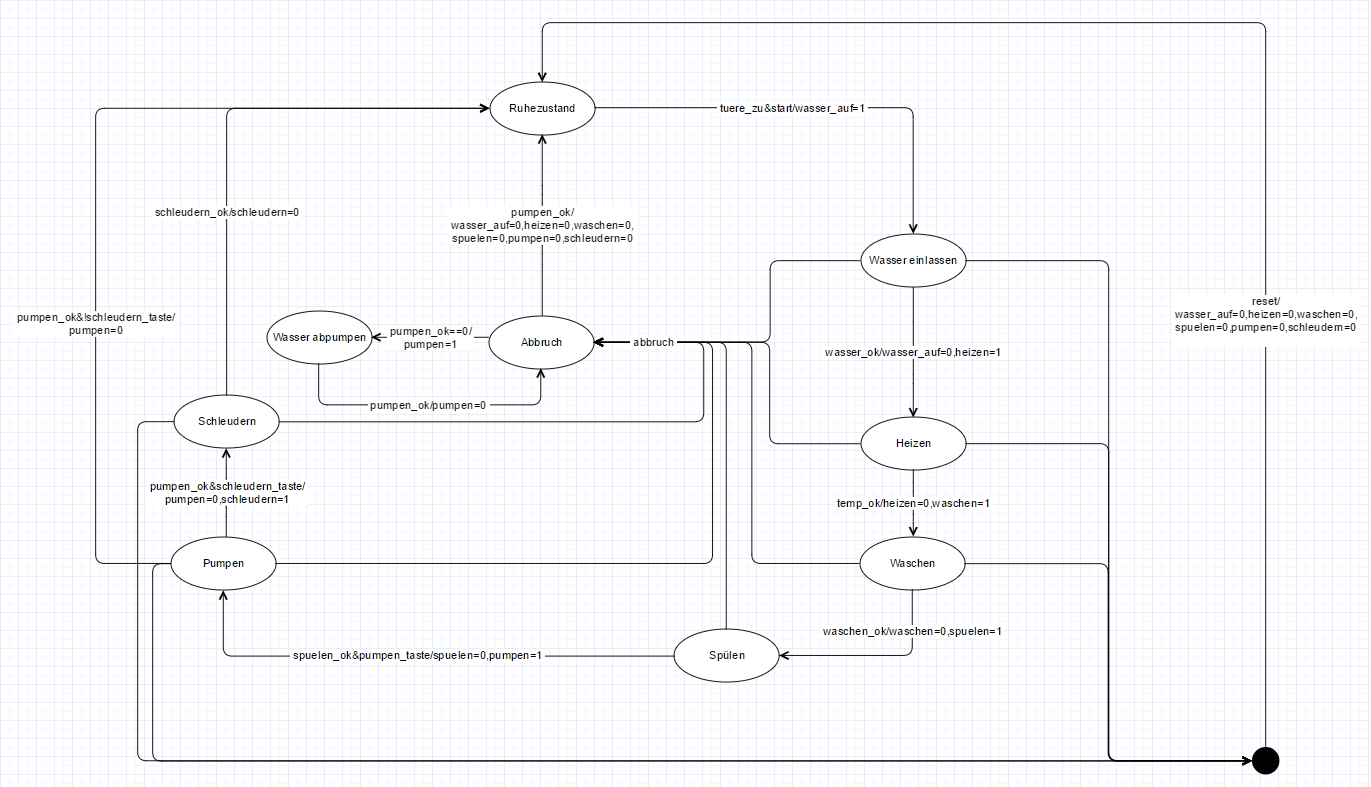
\includegraphics[width = 1.0\textwidth]{waschmaschine_fsm}
		\item VCD Waves
		
		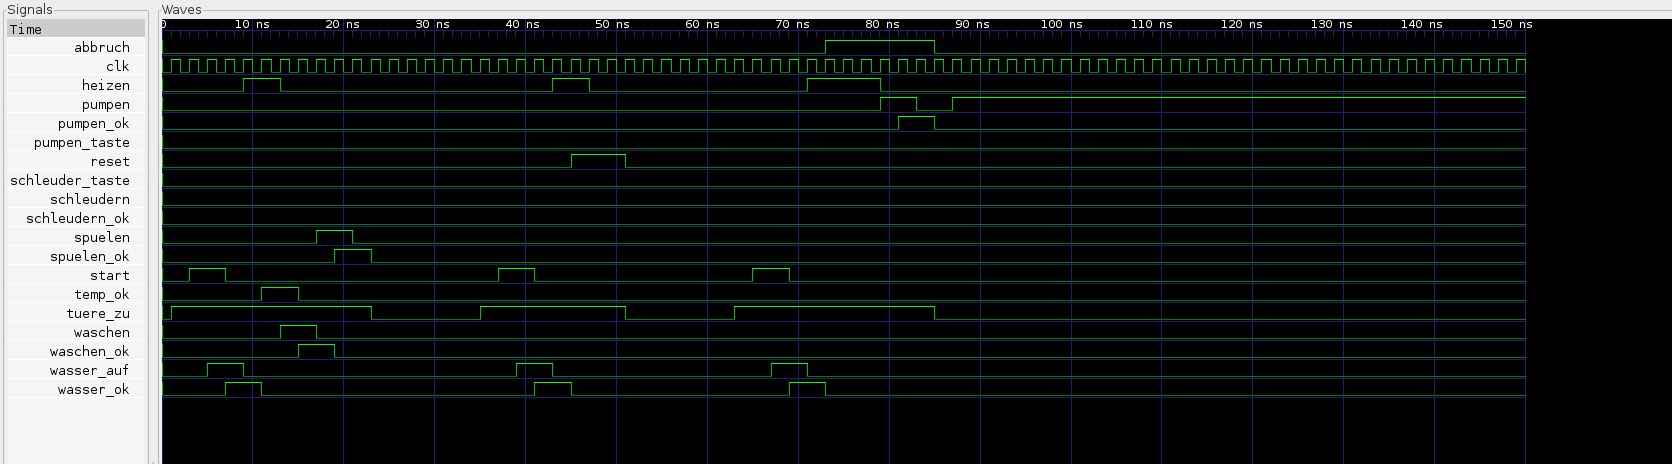
\includegraphics[width = 1.0\textwidth]{wave}
		
	\end{enumerate}
	
\end{document}

